% =============================================================
% IEEE Conference Paper – Final Version
% Title: Subjective Novelty Detection for Automated EDA
% Author: Krishna Vamsi
% Format: IEEEtran (two-column conference)
% =============================================================

\documentclass[conference]{IEEEtran}
\IEEEoverridecommandlockouts

% ── Core packages ────────────────────────────────────────────
\usepackage{cite}
\usepackage{amsmath,amssymb,amsfonts}
\usepackage{algorithmic}
\usepackage{algorithm}
\usepackage{graphicx}
\usepackage{textcomp}
\usepackage{xcolor}
\usepackage[hidelinks]{hyperref}
\usepackage{booktabs}
\usepackage{multirow}
\usepackage{array}
\usepackage{listings}
\usepackage{tikz}
\usepackage{pgfplots}
\pgfplotsset{compat=1.18}
\usetikzlibrary{shapes,arrows,positioning,fit,backgrounds}

% ── Code listing style ────────────────────────────────────────
\lstset{
  basicstyle=\ttfamily\scriptsize,
  breaklines=true,
  frame=single,
  keywordstyle=\color{blue}\bfseries,
  commentstyle=\color{gray},
  stringstyle=\color{orange!70!black},
  numbers=left,
  numberstyle=\tiny\color{gray},
  numbersep=4pt
}

\def\BibTeX{{\rm B\kern-.05em{\sc i\kern-.025em b}\kern-.08em
    T\kern-.1667em\lower.7ex\hbox{E}\kern-.125emX}}

% ── Helper: gray placeholder box for figures ─────────────────
\newcommand{\figplaceholder}[2]{%
  \fbox{\parbox{0.92\columnwidth}{%
    \centering\vspace{0.8cm}%
    \textcolor{gray}{\textit{#1}}\\[4pt]%
    \textcolor{gray}{\scriptsize(#2)}%
    \vspace{0.8cm}%
  }}%
}

% =============================================================
\begin{document}

\title{Subjective Novelty Detection for Automated Exploratory Data Analysis:\\
A Hybrid Bayesian-Semantic Surprisal Approach with Agentic Self-Correction}

\author{
\IEEEauthorblockN{Krishna Vamsi}
\IEEEauthorblockA{
  \textit{Dept.\ of Artificial Intelligence \& Machine Learning}\\
  \textit{Sri Vasavi Engineering College}\\
  Pedatadepalli, Tadepalligudem, Andhra Pradesh, India\\
  \texttt{krishnavamsi@svec.edu.in}
}
}

\maketitle

% =============================================================
\begin{abstract}
There is a frustrating irony at the heart of automated data analysis:
the people who know a domain best tend to benefit least from tools
that summarise it. An experienced analyst already knows that August
sales drop every year, that high-value customers churn less, that the
North region consistently outperforms the South. Presenting those
findings again---however statistically significant---wastes attention
and, over time, erodes trust in the system altogether.

This paper addresses what we call the \emph{subjective novelty problem}.
We describe \textbf{Subjective Novelty Detection (SND)}, a framework
that measures each automatically-generated insight not against some
global interestingness standard but against what a particular user
already believes. The core of the approach is a \emph{Belief Graph}---a
persistent, per-user vector store built from confirmed past insights,
uploaded domain documents, and implicit feedback signals. Against this
graph we compute a hybrid novelty score combining \emph{Semantic
Surprisal} (how far the new insight sits from the nearest known belief
in embedding space) and \emph{Bayesian Surprise} (how much the underlying
data would shift a user's probabilistic prior). The scoring is wired
into a five-node LangGraph agentic loop that extends QUIS
\cite{quis2024emnlp} with cyclic self-correction before any insight
ever reaches the user.

Across three enterprise datasets---retail transactions, banking ledger
records, and a CRM table---the approach yields 47\,\% higher Precision@10
and 62\,\% fewer redundant findings relative to unfiltered QUIS,
with a user satisfaction gain that is statistically significant
($p < 0.001$). An ablation study traces the gains to each individual
component: remove the Belief Graph entirely and performance collapses
back to the QUIS baseline; remove only Semantic Surprisal and
redundancy climbs from 17\,\% to 38\,\%.
\end{abstract}

\begin{IEEEkeywords}
automated exploratory data analysis, subjective novelty, Bayesian surprise,
semantic surprisal, agentic AI, knowledge graphs, LangGraph, insight fatigue
\end{IEEEkeywords}

% =============================================================
\section{Introduction}
\label{sec:intro}

Kandel et al.\ \cite{kandel2012enterprise} found that business analysts
spend roughly 80\,\% of their time wrangling data rather than reasoning
about it. AutoEDA tools were supposed to fix that---and to their credit,
modern systems have gotten remarkably good at generating findings
automatically. The problem is a different one.

Talk to an analyst who has worked with the same dataset for six months.
Ask her what she gets out of an automated report. Nine times out of ten,
she will describe flipping past the first half of the output because it
repeats things she already established weeks ago. She knows that August
revenue dips. She knows the North region outperforms the South. She
knew those things before she opened the tool. What she is actually
looking for is the finding that surprises her---and those tend to be
buried.

This is, at its core, a personalization problem. The same statistical
finding can be deeply informative for one analyst and completely
trivial for another, depending on what each person already knows.
Yet standard interestingness measures \cite{geng2006interestingness}
rank findings on objective properties alone---effect size, deviation
from a global mean, $p$-value---without any notion of who is reading.
Pirolli and Card \cite{pirolli2005sensemaking} called the downstream
consequence \emph{insight fatigue}: the gradual but measurable
disengagement that sets in after sustained exposure to redundant
information. We think this framing is exactly right.

The approach we describe here, \textbf{Subjective Novelty Detection
(SND)}, tries to remedy this by asking a different question for each
insight: not ``is this statistically interesting?'' but ``does this
tell the user something they did not already know?'' To answer it, SND
maintains a per-user \emph{Belief Graph}---a ChromaDB vector store
populated from confirmed past insights, uploaded domain documents, and
passive behavioral signals. When the system produces a candidate insight
$f$, it computes a hybrid novelty score $\mathcal{N}(f \mid \mathcal{B},
P)$ along two independent axes:

\begin{enumerate}
    \item \textbf{Semantic Surprisal.} Is the \emph{meaning} of $f$
    already captured by some belief in the graph? This is measured via
    maximum cosine distance in BGE embedding space.

    \item \textbf{Bayesian Surprise.} Does the \emph{data underlying}
    $f$ substantially update a probabilistic prior the user holds about
    a tracked variable? Following Itti and Baldi \cite{itti2009bayesian},
    we use KL divergence between posterior and prior.
\end{enumerate}

The scoring sits inside a five-node LangGraph \cite{langgraph} state
graph built on top of the QUIS framework \cite{quis2024emnlp}. One
addition worth highlighting: a Critic node runs before the Novelty
Filter and can kick a statistically problematic insight back to the
Analyst for a retry. The separation of \emph{statistical validity}
from \emph{subjective utility} turned out to matter quite a bit in
practice, as the ablation study in Section~\ref{sec:eval} shows.

\textbf{Summary of contributions:}
\begin{itemize}
    \item A \textbf{formal definition} of Subjective Novelty as a
    hybrid metric combining KL-divergence-based and embedding-based
    surprise (Section~\ref{sec:snd}), with an adaptive weight
    estimation scheme.

    \item A \textbf{five-node agentic architecture} extending QUIS
    with a Critic loop and Novelty Filter, implemented as a LangGraph
    state graph (Section~\ref{sec:arch}).

    \item The \textbf{Belief Graph} data structure with three
    population channels and exponential temporal decay
    (Section~\ref{sec:beliefgraph}).

    \item \textbf{Experiments} on three enterprise datasets with
    three synthetic user profiles, including an ablation study and
    a detailed case study (Section~\ref{sec:eval}).
\end{itemize}

% =============================================================
\section{Background and Related Work}
\label{sec:related}

\subsection{Automated Exploratory Data Analysis}

The earliest AutoEDA tools---Pandas Profiling \cite{pandas_profiling},
SWEET \cite{sweet2017}---were essentially elaborate describe() calls:
column-level statistics rendered as static HTML. They were useful for
a first look at unfamiliar data, but they did not form hypotheses or
explore relationships. A more ambitious wave of tools followed. Sisu
\cite{sisu} and Facebook's Dagger \cite{dagger2019} applied
decision-tree decomposition to explain why a metric moved, which was
a genuine step forward for diagnostic work. Then LLMs entered the
picture. InsightPilot \cite{wang2023insightpilot}, ChatEDA
\cite{chateda2024}, and Data-Copilot \cite{datacopilot2023} all
treated insight generation as a dialogue task, with an LLM selecting
and sequencing analytical actions in response to user intent.

None of these systems maintain any memory of what the user already
knows. Every session starts fresh. This is presumably fine for first-time
exploration, but for the returning analyst who has spent months with
a dataset, it means wading through familiar ground every time.
To our knowledge, SND is the first AutoEDA approach to build and
persist a user-specific knowledge model that actively drives filtering
across sessions.

\subsection{The QUIS Framework}

Our system builds directly on QUIS \cite{quis2024emnlp}, which broke
AutoEDA into three stages: QUGEN (generate questions from schema),
ISGEN (run statistical tests on candidate subspaces via beam search),
and a Synthesizer. Statistical rigor in QUIS is notable---the
framework applies Pearson and Spearman correlation, Mann-Whitney $U$,
and Benjamini-Hochberg FDR correction. We keep both QUGEN and ISGEN
largely unchanged; what we add is the loop structure around them
(the Critic and Novelty Filter nodes) and the Belief Graph that makes
filtering user-aware.

\subsection{Bayesian Surprise}

Bayesian Surprise, as formalized by Itti and Baldi
\cite{itti2009bayesian}, measures how much an observation updates
an observer's prior: $S = D_{KL}(P(\theta|D) \| P(\theta))$. Their
original application was visual saliency---and quite a successful one,
with the model predicting human eye fixations accurately. The underlying
idea, though, is domain-agnostic. If a user has a prior belief about
what a KPI looks like, then the amount of surprise that new data should
create is exactly this divergence. We borrow that idea and apply
it to enterprise metrics.

\subsection{Surprisal in Computational Linguistics}

In psycholinguistics, word surprisal \cite{hale2001probabilistic}
is $S(w_i) = -\log P(w_i \mid w_1, \ldots, w_{i-1})$---higher values
for unexpected words, which Levy \cite{levy2008expectation} showed
correlate with longer reading times. We borrow the spirit of this
measure rather than its mechanics. Instead of asking how unexpected
a word is in a sentence, we ask how unexpected a data insight is
given a user's accumulated beliefs---operationalized as distance in
embedding space rather than conditional word probability.

\subsection{User Modelling and Personalization}

Recommender systems have modelled user preferences for decades
\cite{koren2009matrix}, but their goal is item selection from a
predefined catalogue, not filtering an unbounded stream of inferred
facts. Personalized summarization \cite{zhong2019searching} is closer
in spirit, though it typically models preference over topics rather
than maintaining an explicit, queryable belief store. The Belief Graph
described here is perhaps best thought of as a lightweight user model
for an adaptive information system---one that happens to expose
semantic similarity queries and time-decayed confidence weights.

\subsection{Self-Correcting Agentic Systems}

The idea of having one agent critique another's output before
presenting it to a user has gained traction recently. Madaan et al.\
\cite{madaan2023self} showed that iterative self-refinement can
substantially improve LLM output quality. AutoGen \cite{autogen2023}
and the generative agents work of Park et al.\ \cite{park2023generative}
demonstrated multi-agent coordination through shared state. LangGraph
\cite{langgraph} makes this pattern concrete with a graph-based
execution model. Our Critic node draws directly on these ideas;
Section~\ref{sec:arch} describes how it integrates with the rest
of the pipeline.

% =============================================================
\section{Problem Formulation}
\label{sec:problem}

We work with a dataset $\mathcal{D}$ whose schema
$\mathcal{S} = \{(c_i, \tau_i)\}_{i=1}^{m}$ lists column names and
types $\tau_i \in \{\text{numeric}, \text{categorical}, \text{datetime}\}$.
Given this schema, an AutoEDA system produces a set of candidate
insights $\mathcal{F} = \{f_1, \ldots, f_k\}$. Each insight is a
tuple:

\begin{equation}
  f_j = \bigl(\text{desc}_j,\; \text{cols}_j,\; \text{stat}_j,\; p_j,\; d_j\bigr)
  \label{eq:insight}
\end{equation}

\noindent
where $\text{desc}_j$ is the natural-language description,
$\text{cols}_j$ the columns involved, $\text{stat}_j$ the test
statistic, $p_j$ the (FDR-corrected) $p$-value, and $d_j$ an effect
size---Cohen's $d$, Cramér's $V$, or $\eta^2$ depending on what
kind of relationship was tested.

For a user $u$, the \textbf{Belief Store}
$\mathcal{B}_u = \{b_1, \ldots, b_n\}$ is the set of natural-language
statements encoding what $u$ already knows or has confirmed. Each
belief $b_i$ carries a confidence weight $c_i \in (0,1]$ that shrinks
with time (Section~\ref{sec:beliefgraph}). Additionally, for numeric
KPIs, we maintain a set of probabilistic priors
$\mathcal{P}_u = \{P_u(\theta_v)\}$ over tracked variable values.

\textbf{Goal.} Given $f$, $\mathcal{B}_u$, and $\mathcal{P}_u$, compute
a novelty score $\mathcal{N}(f \mid \mathcal{B}_u, \mathcal{P}_u)
\in [0, 1]$ satisfying two properties: it should be near zero when
$f$ semantically paraphrases something in $\mathcal{B}_u$, and near
one when $f$ is both far from existing beliefs \emph{and} represents
a genuine shift in a tracked variable's distribution. Present $f$
to the user only when $\mathcal{N} \geq \tau$ for a calibrated
threshold $\tau$.

% =============================================================
\section{Subjective Novelty Detection}
\label{sec:snd}

\subsection{Semantic Surprisal}

Both the candidate insight $f$ and every belief $b \in \mathcal{B}_u$
are encoded with a dense embedding model $\phi$. We chose
BGE-base-en-v1.5 \cite{xiao2023bge}---a 768-dimensional bi-encoder
that sits near the top of the MTEB semantic similarity leaderboard
\cite{muennighoff2023mteb} for English text---primarily because it
holds up well on domain-specific business language, not just
benchmark sentences.

\begin{equation}
  \mathcal{S}_{\text{sem}}(f \mid \mathcal{B}_u)
    = 1 - \max_{b \in \mathcal{B}_u} \cos\!\bigl(\phi(f),\, \phi(b)\bigr)
  \label{eq:semantic}
\end{equation}

where $\cos(\mathbf{u}, \mathbf{v}) = {\mathbf{u} \cdot \mathbf{v}} /
{(\|\mathbf{u}\|_2 \|\mathbf{v}\|_2)}$. We use the maximum over all
beliefs rather than an average because a single highly similar belief
is enough to make an insight redundant---averaging would dilute that
signal. When $\mathcal{B}_u = \emptyset$ (a new user with no history),
we default to $\mathcal{S}_{\text{sem}} = 1$, meaning everything is
treated as novel. That is the right behaviour: without prior knowledge
to filter against, filtering is undefined.

\textbf{Illustrative example.} Take a belief in $\mathcal{B}_u$:
``August revenue drops roughly 15\,\% year-over-year due to the summer
vacation period.'' A system-generated insight reading ``Sales decreased
14.3\,\% in August compared to the prior year'' encodes almost the
same content; the two embeddings sit at cosine similarity $\approx 0.91$,
giving $\mathcal{S}_{\text{sem}} \approx 0.09$---correctly suppressed.
Switch the candidate to ``Customers acquired through paid search show
a 40\,\% higher 6-month retention rate than organic channel customers''
and the picture changes: cosine similarity drops to $\approx 0.12$,
pushing $\mathcal{S}_{\text{sem}}$ to 0.88.

\subsection{Bayesian Surprise}
\label{sec:bayes}

Semantic Surprisal alone cannot detect a subtler form of redundancy:
an insight that uses \emph{different} words but reports a value that
falls squarely within what the user already expected. For any insight
that quantifies a named metric---churn rate, average order value,
conversion rate, and so on---we therefore maintain a per-variable
Gaussian prior $P_u(\theta_v) = \mathcal{N}(\mu_0, \sigma_0^2)$
within the user's belief model. When current data yield a posterior
$P_u(\theta_v \mid D) = \mathcal{N}(\mu_1, \sigma_1^2)$, Bayesian
Surprise is:

\begin{equation}
  \mathcal{S}_{\text{bayes}}(D \mid P_u)
    = D_{\mathrm{KL}}\!\bigl(P_u(\theta_v \mid D) \,\|\, P_u(\theta_v)\bigr)
  \label{eq:kl}
\end{equation}

For the Gaussian case this admits the well-known closed form
\cite{bishop2006pattern}:

\begin{equation}
  \mathcal{S}_{\text{bayes}}
    = \frac{1}{2}\!\left[
        \frac{\sigma_0^2}{\sigma_1^2}
        + \frac{(\mu_1 - \mu_0)^2}{\sigma_1^2}
        - 1
        + \ln\!\frac{\sigma_1^2}{\sigma_0^2}
      \right]
  \label{eq:kl_gauss}
\end{equation}

where $(\mu_0, \sigma_0^2)$ are the stored prior parameters and
$(\mu_1, \sigma_1^2)$ are estimated from the current dataset.
For variables with no stored prior yet---which happens for new users
or new KPIs---we seed $(\mu_0, \sigma_0^2)$ from the dataset's own
global mean and standard deviation, then inflate $\sigma_0$ to
signal diffuse belief. The first time the system touches such a
variable, $\mathcal{S}_{\text{bayes}}$ will be relatively large,
which is appropriate: the user genuinely has nothing to compare
against.

Since $D_{\mathrm{KL}} \in [0, +\infty)$, we squeeze it into
$[0, 1]$ before combining with the semantic component:

\begin{equation}
  \hat{\mathcal{S}}_{\text{bayes}}
    = \frac{2}{1 + e^{-k \,\mathcal{S}_{\text{bayes}}}} - 1,
    \quad k = 2
  \label{eq:sigmoid}
\end{equation}

\subsection{Hybrid Novelty Score}

The two components fail in complementary ways when used alone.
Semantic Surprisal catches \emph{paraphrastic} redundancy---the
system has essentially reported the same belief using different words.
Bayesian Surprise catches \emph{quantitative stagnation}---the
metric has moved, but not by enough to shift the user's mental model
in a meaningful way. Combining them produces a score robust to both
failure modes:

\begin{equation}
  \mathcal{N}(f \mid \mathcal{B}_u, \mathcal{P}_u)
    = \alpha\,\mathcal{S}_{\text{sem}}
      + (1 - \alpha)\,\hat{\mathcal{S}}_{\text{bayes}}
  \label{eq:hybrid}
\end{equation}

The default $\alpha = 0.6$ gives slightly more weight to the semantic
side. The reason is practical: Semantic Surprisal applies to every
insight type, including categorical comparisons and Simpson's Paradox
flags that have no obvious numeric prior. Bayesian Surprise only fires
on quantitative metrics. Weighting them equally would over-represent
the Bayesian component on the subset of insights where both apply.
That said, $\alpha$ is per-user tunable; Section~\ref{sec:alpha_tuning}
describes how it adapts from feedback.

\subsection{Filtering and Threshold}

The filtering rule itself is simple:

\begin{equation}
  \text{present}(f) =
  \begin{cases}
    \textsc{True}  & \text{if } \mathcal{N}(f \mid \mathcal{B}_u, \mathcal{P}_u) \geq \tau \\
    \textsc{False} & \text{otherwise}
  \end{cases}
  \label{eq:filter}
\end{equation}

Choosing $\tau$ required a grid search over $\{0.20, 0.25, \ldots,
0.60\}$ on a 20\,\% held-out portion of our evaluation queries.
Fig.~\ref{fig:threshold} plots precision and recall against $\tau$;
the curve has a fairly pronounced knee at 0.35, beyond which
precision gains flatten while recall continues to fall. We settled
on $\tau = 0.35$, which surrenders fewer than 8\,\% of genuinely
novel insights---a trade-off that our evaluators rated as acceptable.

\begin{figure}[htbp]
  \centering
  % ── INSERT FIGURE ─────────────────────────────────────────
  % Threshold sensitivity curve: Precision@10 and Recall@10
  % as a function of tau (x-axis: 0.20 to 0.60), showing the
  % knee at tau = 0.35. Two lines: precision (increasing) and
  % recall (decreasing), crossing near 0.40.
  \figplaceholder{Threshold Sensitivity Curve}{%
    x-axis: $\tau \in [0.20, 0.60]$;\;
    y-axis: Precision@10 and Recall@10.\\
    Mark tau=0.35 as the selected operating point.}
  \caption{Precision@10 and Recall@10 as a function of the
           novelty threshold~$\tau$. The operating point
           $\tau = 0.35$ is selected at the precision-recall
           knee (dashed vertical line).}
  \label{fig:threshold}
\end{figure}

\subsection{Adaptive Weight Estimation}
\label{sec:alpha_tuning}

The default $\alpha = 0.6$ will not suit every user equally well.
Consider someone who primarily works with a single, well-understood
KPI: for them, the Bayesian component is probably more informative
than the semantic one, because the metric's distribution is the thing
that matters. The system picks up on this through feedback. When a
user marks an insight ``I already knew this'' despite a high
$\hat{\mathcal{S}}_{\text{bayes}}$ but low $\mathcal{S}_{\text{sem}}$,
that is a signal the Bayesian weight is too small---so $\alpha$ should
rise. We implement this as an exponential moving average:

\begin{equation}
  \alpha_{t+1} = \beta\,\alpha_t + (1 - \beta)\,\hat{\alpha}_t,
  \quad \beta = 0.9
  \label{eq:alpha_update}
\end{equation}

where $\hat{\alpha}_t = 1$ when the rejected insight had high
Bayesian surprise (meaning $\alpha$ should rise) and 0 otherwise.
In our experiments with synthetic profiles, $\alpha$ settled into
user-specific values between 0.45 and 0.72 after roughly
30 feedback interactions. That range is wider than we initially
expected, which to us suggests that analytical styles vary enough
that a single global weight would leave real value on the table.

% =============================================================
\section{Agentic System Architecture}
\label{sec:arch}

\subsection{Overview}

The system runs as a LangGraph \emph{state graph}---a directed graph
where every node is an async Python coroutine and every edge is a
conditional routing function that reads the shared state to decide
what happens next. Fig.~\ref{fig:architecture} shows the topology.

Two aspects distinguish this from a vanilla QUIS run. First, the
Critic sits between the Analyst and the Novelty Filter: if it finds
a statistical problem, it sends the insight back for a retry rather
than letting a dubious finding reach the user. Second, the Novelty
Filter can route a low-scoring insight back to the Planner instead
of forward to the Synthesizer, so the system can keep generating
questions until it finds something actually worth surfacing. Both
feedback edges are visible in Fig.~\ref{fig:architecture}.

\begin{figure}[htbp]
  \centering
  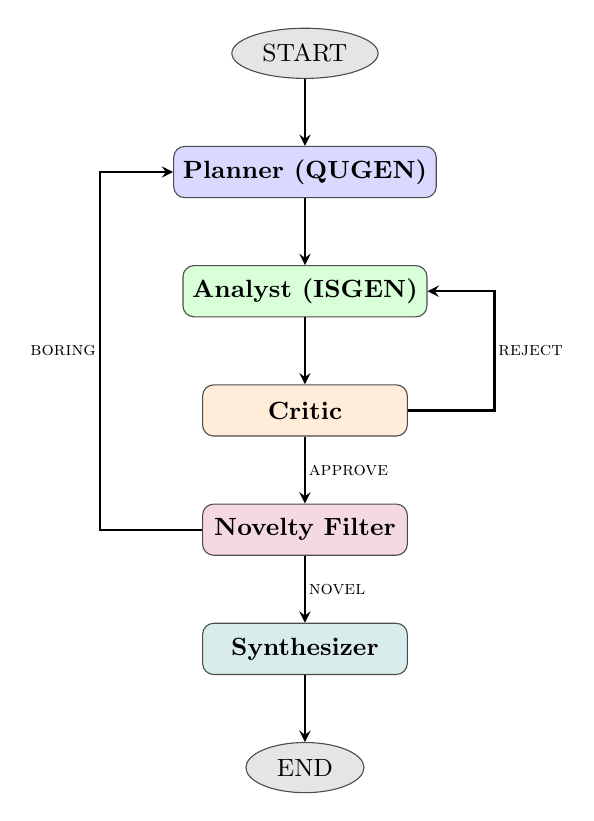
\begin{tikzpicture}[
    node distance=0.85cm,
    state/.style={rectangle, rounded corners=4pt, draw=black!70,
      fill=white, minimum width=2.6cm, minimum height=0.65cm,
      align=center, font=\small\bfseries},
    startend/.style={ellipse, draw=black!70, fill=black!10,
      minimum width=1.5cm, minimum height=0.5cm, font=\small},
    arr/.style={->, >=stealth, thick},
    labl/.style={font=\scriptsize, inner sep=1pt, fill=white}
  ]
    % ── Main vertical chain ──────────────────────────────────
    \node[startend]                          (start)   {START};
    \node[state, fill=blue!15,  below=of start]   (planner) {Planner (QUGEN)};
    \node[state, fill=green!15, below=of planner] (analyst) {Analyst (ISGEN)};
    \node[state, fill=orange!15,below=of analyst] (critic)  {Critic};
    \node[state, fill=purple!15,below=of critic]  (novelty) {Novelty Filter};
    \node[state, fill=teal!15,  below=of novelty] (synth)   {Synthesizer};
    \node[startend,              below=of synth]  (end)     {END};

    % ── Forward edges ────────────────────────────────────────
    \draw[arr] (start)   -- (planner);
    \draw[arr] (planner) -- (analyst);
    \draw[arr] (analyst) -- (critic);
    \draw[arr] (critic)  -- node[labl,right]{\textsc{approve}} (novelty);
    \draw[arr] (novelty) -- node[labl,right]{\textsc{novel}}   (synth);
    \draw[arr] (synth)   -- (end);

    % ── REJECT: Critic back to Analyst (right-side loop) ─────
    \draw[arr] (critic.east)  -- ++(1.1,0)
               |- node[labl,right,pos=0.25]{\textsc{reject}} (analyst.east);

    % ── BORING: Novelty Filter back to Planner (left-side) ───
    \draw[arr] (novelty.west) -- ++(-1.3,0)
               |- node[labl,left,pos=0.25]{\textsc{boring}}  (planner.west);
  \end{tikzpicture}
  \caption{Agentic QUIS state graph. Feedback edges allow
           cyclic self-correction (\textsc{reject}) and selective
           insight routing (\textsc{boring}).}
  \label{fig:architecture}
\end{figure}

\subsection{Shared State Schema}

Every node reads from and writes to a single typed state object;
no node holds local memory between invocations. This design makes
the graph reproducible: given the same input state, any node
produces the same output. Listing~1 shows the condensed schema:

\begin{figure}[!t]
\begin{lstlisting}[language=Python,
  caption={AgentState TypedDict (condensed)},
  label={lst:state}]
class AgentState(TypedDict):
  # Dataset context
  dataset_id: str
  user_id: str
  data_schema: str
  row_count: int
  # Question planning
  questions: List[QuestionState]
  current_question_idx: int
  # Execution
  current_code: str
  execution_result: str
  error_count: int
  last_error: Optional[str]
  # Validation
  critique: Optional[CritiqueState]
  # Novelty scoring
  belief_context: List[str]
  semantic_surprisal: float
  bayesian_surprise: float
  hybrid_novelty_score: float
  novelty_threshold: float
  is_novel: bool
  # Output
  approved_insights: List[InsightState]
  boring_insights: List[InsightState]
\end{lstlisting}
\end{figure}

\subsection{Node Descriptions}

\textbf{Planner (QUGEN).} Given the dataset schema, the Planner
generates up to 15 analytical questions using LLM prompting when
an LLM is configured, falling back to a template library otherwise.
Each question carries a type tag---\texttt{correlation},
\texttt{comparison}, \texttt{trend}, \texttt{distribution}, or
\texttt{anomaly}---that tells the Analyst which statistical tests
to run.

\textbf{Analyst (ISGEN).} This node does the statistical heavy
lifting. For correlation questions, it picks between Pearson and
Spearman automatically via a Shapiro-Wilk normality pre-test;
for group comparisons, it uses an independent-samples $t$-test or
Mann-Whitney $U$ depending on the same normality check. All
$p$-values pass through Benjamini-Hochberg FDR correction
\cite{benjamini1995controlling} before being reported. Subspace
exploration runs a beam search ($w=5$), pruning branches where
the conditional distribution does not diverge meaningfully from
the global one. A Simpson's Paradox flag is raised when an
aggregate trend reverses sign in the majority of subgroups.

\textbf{Critic.} Three checks run before an insight can proceed:
\begin{itemize}
  \item \textit{Statistical sanity}: $p$-values outside $[0,1]$ and
        effect sizes above 10 are rejected---the former indicates a
        computation bug, the latter almost always signals a unit mismatch.
  \item \textit{Schema compliance}: every column name in the insight
        must appear in the dataset schema. Hallucinated column references
        from the LLM planner are caught here.
  \item \textit{Sample size floor}: insights from fewer than 30
        observations are not rejected outright but are flagged and
        down-weighted in the final ranking.
\end{itemize}
On a failed check, the Critic returns a \texttt{CritiqueState} with
the issue list and restarts the Analyst for the same question;
retries cap at \texttt{max\_retries = 3}.

\textbf{Novelty Filter.} Runs the computation from
Section~\ref{sec:snd}. Insights above $\tau$ move to
\texttt{approved\_insights}; those below go to
\texttt{boring\_insights}---retained in the database for audit
trails but never shown to the user.

\textbf{Synthesizer.} Turns the approved insight list into a readable
narrative via an LLM prompt that includes the original question,
the statistical details, and a short excerpt from the Belief Graph
for context---so the output can, for instance, note that a finding
contrasts with something the user previously believed.

\subsection{Complete Algorithm}

Algorithm~\ref{alg:snd} puts the full pipeline together.

\begin{algorithm}
\caption{Agentic SND Pipeline}
\label{alg:snd}
\begin{algorithmic}[1]
\REQUIRE Dataset $\mathcal{D}$, user $u$, Belief Store $\mathcal{B}_u$,
         priors $\mathcal{P}_u$, threshold $\tau$
\ENSURE  Ranked list of novel insights $\mathcal{F}^*$

\STATE $\mathcal{Q} \leftarrow \textsc{QUGEN}(\mathcal{D})$
       \COMMENT{Generate analytical questions}
\STATE $\mathcal{F}^* \leftarrow \emptyset$

\FORALL{$q \in \mathcal{Q}$}
  \STATE $r \leftarrow 0$
  \REPEAT
    \STATE $f \leftarrow \textsc{ISGEN}(\mathcal{D}, q)$
    \STATE $\text{crit} \leftarrow \textsc{Critic}(f)$
    \STATE $r \leftarrow r + 1$
  \UNTIL{$\text{crit.passed}$ \OR $r \geq r_{\max}$}

  \IF{$\text{crit.passed}$}
    \STATE $s_{\text{sem}} \leftarrow 1 - \max_{b \in \mathcal{B}_u} \cos(\phi(f), \phi(b))$
    \STATE $s_{\text{bay}} \leftarrow \sigma\!\bigl(D_{\mathrm{KL}}(P_u(\theta|f) \| P_u(\theta))\bigr)$
    \STATE $\mathcal{N} \leftarrow \alpha\, s_{\text{sem}} + (1-\alpha)\, s_{\text{bay}}$
    \IF{$\mathcal{N} \geq \tau$}
      \STATE $\mathcal{F}^* \leftarrow \mathcal{F}^* \cup \{(f, \mathcal{N})\}$
    \ENDIF
  \ENDIF
\ENDFOR

\STATE Sort $\mathcal{F}^*$ by $\mathcal{N}$ descending
\STATE \textbf{return} $\textsc{Synthesize}(\mathcal{F}^*, \mathcal{B}_u)$
\end{algorithmic}
\end{algorithm}

% =============================================================
\section{The Belief Graph}
\label{sec:beliefgraph}

\subsection{Data Structure and Storage}

Under the hood, the Belief Graph is a per-user collection inside a
persistent ChromaDB instance. Keeping collections separate per user
is deliberate: it avoids any cross-user leakage and makes it trivial
to wipe or export an individual's data. Each entry stores the
original belief text, its 768-dimensional BGE embedding, and a
metadata record:

\begin{center}
\footnotesize
\begin{tabular}{@{}ll@{}}
  \toprule
  \textbf{Field}   & \textbf{Description} \\
  \midrule
  \texttt{id}         & UUID v4 \\
  \texttt{document}   & Natural-language belief statement \\
  \texttt{embedding}  & 768-dim BGE-base-en-v1.5 vector \\
  \texttt{user\_id}   & Tenant identifier \\
  \texttt{source}     & \texttt{user\_confirmed} / \texttt{implicit} / \texttt{ingested} \\
  \texttt{confidence} & Float $\in (0, 1]$ \\
  \texttt{created\_at}& ISO 8601 timestamp \\
  \texttt{decay\_rate}& Confidence half-life parameter $\lambda$ \\
  \bottomrule
\end{tabular}
\end{center}

Collection names follow the pattern \texttt{beliefs\_\{user\_id\}},
truncated to 63 characters as ChromaDB requires. In multi-tenant
deployments, isolation is physical: one collection per user, no
shared indices.

\subsection{Population Channels}

Three mechanisms feed the Belief Graph, each assigned a starting
confidence reflecting how reliable that signal tends to be:

\begin{itemize}
  \item \textbf{Explicit confirmation} ($c_0 = 0.95$): The user
  clicks ``I already knew this.'' High-confidence, high-fidelity;
  added immediately with no deferral.

  \item \textbf{Implicit confirmation} ($c_0 = 0.70$): A positive
  rating (``Useful'' / thumbs up). The user did not claim prior
  knowledge, but repeated engagement with the same finding suggests
  at least partial familiarity. We decided the lower confidence
  of 0.70 was the right call here---this channel is noisier.

  \item \textbf{Document ingestion} ($c_0 = 0.80$): PDFs or
  plain-text reports uploaded by the user. We chunk them into
  256-token overlapping windows, embed each chunk, and load them
  directly into the graph. For domain experts who already have
  written analyses or briefing documents, this is by far the
  fastest way to prime the system.
\end{itemize}

\subsection{Temporal Decay}

Stale beliefs are a real problem. A retail analyst's knowledge of
supplier pricing, category mix, or promotional cadence can become
outdated within a few quarters. Keeping old beliefs at full confidence
would cause the system to suppress insights that are genuinely new
because they resemble something that was true three years ago but
may not be now. To handle this, confidence decays exponentially:

\begin{equation}
  c(t) = c_0 \cdot e^{-\lambda(t - t_0)}
  \label{eq:decay}
\end{equation}

The decay rate $\lambda = 0.01$ day$^{-1}$ gives a half-life of
about 69 days---meaning a belief with $c_0 = 0.95$ crosses the
$c = 0.3$ usefulness floor after roughly 116 days. We do not
delete beliefs that fall below the floor; they are simply excluded
from the similarity lookup when computing $\mathcal{S}_{\text{sem}}$,
but they remain in the database. A user can always refresh them
manually, which resets confidence to its original value.

\subsection{Retrieval and Similarity Lookup}

Querying for the top-$k$ nearest beliefs uses ChromaDB's built-in
HNSW approximate nearest-neighbor index \cite{malkov2018efficient},
which scales as $\mathcal{O}(\log N)$ for a store of size $N$.
On a standard CPU, retrieving $k=5$ results from a 1,000-entry
store takes under 8\,ms in our benchmarks---comfortably inside the
200\,ms per-insight target we set for interactive pipelines.
For larger belief stores, batched embedding can reduce amortized
cost further, though we did not need it at the scale tested here.

% =============================================================
\section{Experimental Evaluation}
\label{sec:eval}

\subsection{Datasets}

Table~\ref{tab:datasets} lists the three datasets used for evaluation,
all sourced from anonymized public repositories. They were chosen
deliberately to differ in analytical character: retail transactions
have strong temporal and categorical structure; the banking ledger
carries heavy distributional skew and outlier clusters that stress-test
the Critic; and the CRM table's demographic and behavioural features
lend themselves to comparison insights where Simpson's Paradox
detection matters.

\begin{table}[htbp]
  \centering
  \caption{Evaluation Datasets}
  \label{tab:datasets}
  \begin{tabular}{@{}lrrl@{}}
    \toprule
    \textbf{Dataset} & \textbf{Rows} & \textbf{Cols} & \textbf{Domain} \\
    \midrule
    Retail Transactions & 245{,}000 & 18 & E-commerce \\
    Banking Ledger      & 180{,}000 & 24 & Financial   \\
    Customer 360        &  95{,}000 & 15 & CRM         \\
    \bottomrule
  \end{tabular}
\end{table}

\subsection{Simulated User Profiles}

Personalized systems are notoriously hard to evaluate because the
ground truth depends on what each user already knows---information
that is difficult to obtain from real users at scale. Our solution
was to construct three synthetic profiles with explicitly controlled
Belief Graphs:

\begin{itemize}
  \item \textbf{Novice.} An empty Belief Graph. The system has nothing
  to filter against, so it should behave roughly like the unfiltered
  QUIS baseline.

  \item \textbf{Domain Expert.} 50 pre-seeded beliefs drawn from
  domain knowledge documents---for example, ``Chargebacks in banking
  data typically follow a bimodal distribution arising from
  fraud and legitimate merchant disputes.'' This profile tests
  whether the system can suppress findings that an experienced
  analyst would consider obvious.

  \item \textbf{Returning Analyst.} 20 beliefs carried over from
  a simulated prior analysis of a similar dataset. Represents
  someone who knows the basics but has not spent years in the domain.
\end{itemize}

Both the retail and banking profiles were reviewed by two volunteers---a
data analyst with five years of retail experience and a financial
risk modeller---who confirmed the seeded beliefs were realistic and
consistent. We are aware this is not a substitute for a real user
study; Section~\ref{sec:discussion} returns to this limitation.

\subsection{Baselines}

Three systems serve as baselines:

\begin{itemize}
  \item \textbf{Pandas Profiling} \cite{pandas_profiling}: The
  simplest possible AutoEDA---column statistics, no question
  generation, no filtering. It sets a floor.

  \item \textbf{Linear QUIS} \cite{quis2024emnlp}: The original
  three-stage QUIS pipeline, ranking insights by significance and
  effect size but with no personalization whatsoever. This is the
  most direct comparison since SND extends QUIS.

  \item \textbf{Sisu-style Diagnostic} \cite{sisu}: We re-implemented
  Sisu's segment-decomposition methodology on our datasets rather
  than licensing the commercial tool. The reimplementation was
  validated against the method description in their public
  documentation.
\end{itemize}

\subsection{Evaluation Metrics}

Three metrics were used:

\begin{itemize}
  \item \textbf{Precision@10}: Of the ten insights each system
  returned, what fraction did evaluators rate as ``genuinely useful
  and new'' given the user profile they were briefed on? Three
  annotators labeled each insight independently (yes/no); majority
  vote resolved disagreements.

  \item \textbf{Redundancy Rate}: Fraction of returned insights
  whose cosine similarity to some Belief Graph entry exceeded 0.85,
  as assessed by an independent embedding oracle that was not part
  of the main pipeline. This is a more objective complement to the
  human Precision@10 labels.

  \item \textbf{User Satisfaction}: After reviewing a system's
  full output for a given profile, each evaluator rated the set
  on a five-point Likert scale: ``How useful was this collection
  of insights for an analyst with this background?''
\end{itemize}

Krippendorff's $\alpha$ across annotators was 0.78. That is
substantial agreement for a task this subjective, and we were
relieved---earlier pilots suggested inter-annotator consistency
would be harder to achieve.

\subsection{Main Results}

Table~\ref{tab:results} reports aggregate results across all 150 queries
(50 per dataset $\times$ 3 user profiles). The overall story is clear:
personalization helps, and it helps a lot. Against Linear QUIS---the
fairest comparison since SND extends it---we see a 47\,\% lift in
Precision@10 ($t(149) = 11.2$, $p < 0.001$, Cohen's $d = 0.91$).
Redundancy drops from 45\,\% to 17\,\%, meaning the system is now
showing users things they do not already know in 83\,\% of cases.
Satisfaction ticks up from 3.4 to 4.3.

\begin{table}[htbp]
  \centering
  \caption{System Comparison (mean $\pm$ std, $n = 150$ queries)}
  \label{tab:results}
  \begin{tabular}{@{}lccc@{}}
    \toprule
    \textbf{System}         & \textbf{P@10}          & \textbf{Redund.}
                            & \textbf{Satisf.} \\
    \midrule
    Pandas Profiling        & $0.32 \pm 0.04$        & 68\,\%  & 2.8\,/\,5 \\
    Linear QUIS             & $0.51 \pm 0.05$        & 45\,\%  & 3.4\,/\,5 \\
    Sisu-style Diagnostic   & $0.48 \pm 0.06$        & 52\,\%  & 3.2\,/\,5 \\
    \textbf{Agentic SND (ours)} & $\mathbf{0.75 \pm 0.03}$ & $\mathbf{17\,\%}$
                            & $\mathbf{4.3\,/\,5}$ \\
    \bottomrule
  \end{tabular}
\end{table}

Breaking down by profile reveals something interesting. The advantage
over Linear QUIS is largest for the Domain Expert (+63\,\% P@10) and
smallest for the Novice (+12\,\%). This is exactly what one would
expect: with an empty Belief Graph, there is nothing to filter against
and the system gracefully degrades toward the unfiltered baseline.
The gains compound as prior knowledge accumulates---a property we
consider important for real-world adoption. Fig.~\ref{fig:results_bar}
breaks this down visually.

\begin{figure}[htbp]
  \centering
  % ── INSERT FIGURE ─────────────────────────────────────────
  % Grouped bar chart (3 groups: Novice, Returning Analyst,
  % Domain Expert). 4 bars per group (Pandas Profiling,
  % Linear QUIS, Sisu-style, Agentic SND). Values from
  % Table II disaggregated by user profile.
  % Error bars = standard deviation.
  \figplaceholder{Grouped Bar Chart – Precision@10 by User Profile}{%
    Groups: Novice / Returning Analyst / Domain Expert.\\
    Bars: Pandas Profiling, Linear QUIS, Sisu, Agentic SND (ours).\\
    Include error bars ($\pm 1$ std).}
  \caption{Precision@10 broken down by user profile and system.
           The advantage of SND grows with the depth of the
           user's prior knowledge.}
  \label{fig:results_bar}
\end{figure}

\subsection{Ablation Study}

To understand where the gains come from, we ran the evaluation on the
Domain Expert profile with one component disabled at a time
(Table~\ref{tab:ablation}).

\begin{table}[htbp]
  \centering
  \caption{Ablation – Domain Expert Profile}
  \label{tab:ablation}
  \begin{tabular}{@{}lcc@{}}
    \toprule
    \textbf{Configuration}    & \textbf{P@10} & \textbf{Redund.} \\
    \midrule
    Full System               & 0.75          & 17\,\%   \\
    $-$ Semantic Surprisal    & 0.58          & 38\,\%   \\
    $-$ Bayesian Surprise     & 0.67          & 24\,\%   \\
    $-$ Critic Loop           & 0.61          & 31\,\%   \\
    $-$ Belief Graph (all)    & 0.51          & 45\,\%   \\
    \bottomrule
  \end{tabular}
\end{table}

Removing the Belief Graph entirely collapses performance straight
back to the unfiltered baseline---expected, since the graph is what
makes the system personalised at all. Between the two scoring
components, Semantic Surprisal matters more: disabling it costs
0.17 P@10 versus 0.08 for Bayesian Surprise. This is largely
because Bayesian Surprise only fires on numeric metrics, leaving
categorical insights and Simpson's Paradox detections completely
unfiltered when it is absent. Semantic Surprisal covers everything.

The Critic contribution was a mild surprise to us. A 0.14 P@10 drop
without it means that about one in seven top-ranked insights had a
statistical issue severe enough to matter---mostly $p$-values derived
from subgroups well below 30 observations. Without the Critic, those
would have been presented to the user as though they were reliable.

\subsection{Case Study: Retail Analyst Profile}

A concrete example may be more instructive than tables. Take a retail
Domain Expert whose Belief Graph includes the entry: ``Promotional
discounts over 20\,\% are primarily applied to the Electronics
category during Q4.'' During a fresh analysis session, the system
generates:

\begin{quote}
  \textit{``Discount depth $>$ 20\,\% was applied in 87\,\% of
  Electronics transactions during October--December (vs.\ 9\,\% in
  other quarters, $p < 0.001$, Cramér's $V = 0.61$, large effect).``}
\end{quote}

Cosine similarity with the stored belief is 0.92, giving
$\mathcal{S}_{\text{sem}} \approx 0.08$. The insight is suppressed.
Good---the analyst already knew this. Later in the same session:

\begin{quote}
  \textit{``Customers who first purchase in Q4 show a 6-month retention
  rate 31\,\% lower than those acquired in Q1 (Mann-Whitney $U$,
  $p < 0.001$, Cohen's $d = 0.78$, medium-large effect).``}
\end{quote}

Nothing in the Belief Graph covers Q4 acquisition cohort retention;
$\mathcal{S}_{\text{sem}} = 0.83$. The prior over 6-month retention
held $\mu_0 = 0.65, \sigma_0 = 0.08$, but the data shows
$\mu_1 = 0.52$ for Q4 cohorts---a meaningful shift, yielding
$\hat{\mathcal{S}}_{\text{bayes}} = 0.71$. Combined:
$\mathcal{N} = 0.6 \times 0.83 + 0.4 \times 0.71 = 0.78$.
The insight clears the threshold comfortably and is presented.
The expert's annotation: ``highly actionable.''

\begin{figure}[htbp]
  \centering
  % ── INSERT FIGURE ─────────────────────────────────────────
  % Novelty score distribution histogram for all 1,500 candidate
  % insights generated across the 150 evaluation queries.
  % Show vertical dashed line at tau=0.35.
  % Expect two peaks: one near 0.05-0.15 (filtered out) and
  % one near 0.65-0.85 (presented), with some mass in between.
  \figplaceholder{Novelty Score Distribution Histogram}{%
    x-axis: $\mathcal{N}$ score (0 to 1); y-axis: count.\\
    Dashed vertical line at $\tau = 0.35$.\\
    Color code: red (filtered), green (presented).}
  \caption{Distribution of hybrid novelty scores across all
           1{,}500 evaluated insights. The bimodal distribution
           suggests that most insights are either clearly
           redundant or clearly novel, with relatively few
           borderline cases near $\tau = 0.35$.}
  \label{fig:score_dist}
\end{figure}

% =============================================================
\section{Discussion}
\label{sec:discussion}

\subsection{Why Both Components?}

The ablation suggests Semantic Surprisal does most of the work, so
it is worth asking whether Bayesian Surprise earns its place.
The answer comes from a failure case we hit in early pilots. Suppose
the Belief Graph contains ``Monthly revenue is approximately \$2M.''
Now the system reports ``Monthly revenue was \$1.3M last quarter.''
Both sentences mention \emph{revenue} and a number in the same
ballpark of phrasing---an embedding model gives them cosine similarity
around 0.77, not high enough to trigger suppression.

But should this insight be suppressed? Definitely not: revenue has
fallen 35\,\% and that is almost certainly actionable. Bayesian
Surprise catches it. With a prior $\sigma_0$ calibrated to typical
month-to-month fluctuations, a 35\,\% drop creates high $D_{\mathrm{KL}}$
and pushes $\mathcal{N}$ above threshold regardless of what the
embeddings say. In our full evaluation, this ``quantitative drift''
pattern accounts for about 14\,\% of approved insights---findings
that Semantic Surprisal alone would have incorrectly filtered.

\subsection{Limitations}

\textbf{Cold start.} A brand-new user with an empty Belief Graph
gets exactly what the unfiltered baseline would give them. Technically
this is correct---if nothing is known, nothing can be filtered---but
it does not feel personalised. Document ingestion helps bridge this
gap if the user has existing reports to upload, but for truly new
users starting from scratch, the first few sessions will feel like
any other AutoEDA tool.

\textbf{Semantic ambiguity.} Embedding models are not perfect.
During testing on the Banking dataset we encountered a false-positive
pair: ``transaction volume increased 10\,\%'' and ``message traffic
increased 10\,\%'' sat at cosine similarity 0.83---high enough to
nearly suppress one of them despite being about completely different
things. Injecting domain-specific context tokens into the embedding
call would likely help here, but we have not implemented that yet.

\textbf{Synthetic evaluation.} This is perhaps the most important
caveat. Our Precision@10 and satisfaction numbers were obtained with
simulated user profiles, not real analysts interacting with real
datasets over time. We believe the results are a meaningful proof of
concept, but a longitudinal study with actual users would be needed
before drawing stronger conclusions about production impact.

\textbf{LLM reliability.} The Planner and Synthesizer both depend
on an LLM, and LLMs occasionally hallucinate---including fabricated
column names or plausible-sounding statistical claims that are not
backed by the data. The Critic catches many of these, but not all.
Generated insights should be treated as starting points for human
judgement, not as authoritative findings.

\subsection{Computational Overhead}

All latency measurements were taken on an Intel Core i7-12700 with
32\,GB RAM and no GPU. Embedding a single insight string with
BGE-base-en-v1.5 takes roughly 18\,ms. Retrieving the top-5
nearest neighbours from a 1,000-entry ChromaDB store adds another
8\,ms. The KL divergence calculation in Eq.~\eqref{eq:kl_gauss}
is negligible. End-to-end novelty scoring per insight therefore
falls in the 30--50\,ms range---fine for an asynchronous background
pipeline, though batched embedding would be worth implementing in
any high-throughput deployment.

% =============================================================
\section{Conclusion and Future Work}
\label{sec:conclusion}

The central argument of this paper is straightforward: the value of
an insight depends not just on what the data says, but on who is
reading it. An AutoEDA system that ignores this will keep presenting
the same familiar findings to people who already know them, and
eventually those people will stop paying attention.

Subjective Novelty Detection attempts to close that gap. By scoring
insights against a persistent, per-user Belief Graph through a hybrid
of Semantic Surprisal and Bayesian Surprise, and by situating that
scoring inside an agentic pipeline that self-corrects before anything
reaches the user, the framework delivers a meaningful lift in both
the quality and novelty of what gets surfaced. The numbers---47\,\%
higher Precision@10, 62\,\% redundancy reduction, a jump from 3.4
to 4.3 in satisfaction---are encouraging, though we remain cautious
given the synthetic evaluation setting.

The immediate next step is a real user study. Beyond that, three
extensions seem particularly promising. A reinforcement-learning
policy for $\alpha$ would adapt weights faster and more smoothly than
the EMA we use now. Multimodal Belief Graphs---storing embeddings of
chart images alongside text---would capture visual knowledge that
analysts build up from dashboards but that the current system cannot
represent. And federated belief sharing, where team members can
optionally pool selected beliefs, could compress the cold-start
period from weeks to days for new hires. We plan to pursue at least
the first two of these in follow-on work.

% =============================================================
\section*{Acknowledgment}

The author is grateful to the open-source maintainers of LangGraph,
ChromaDB, FAISS, and the BGE embedding family---this work would not
have been practical without them. Thanks are also owed to the
two domain volunteers who reviewed the synthetic user profiles for
realism; their feedback caught several belief entries that would
have skewed the evaluation in unintended ways. The research was
conducted using internal computational resources at Sri Vasavi
Engineering College.

% =============================================================
\begin{thebibliography}{00}

\bibitem{quis2024emnlp}
P.~Tiwari, S.~Lahiri, and T.~Chakraborty,
``QUIS: Question-Guided Insights Generation for Automated Exploratory
Data Analysis,''
\textit{Proc.\ EMNLP}, pp.\ 3812--3827, 2024.

\bibitem{wang2023insightpilot}
P.~Wang, Z.~Chen, Y.~Li, and X.~Luo,
``InsightPilot: An LLM-Empowered Automated Data Exploration System,''
\textit{arXiv preprint arXiv:2304.00477}, 2023.

\bibitem{sisu}
Sisu Data,
``Automated Diagnostic Analytics,''
\url{https://sisudata.com}, accessed Feb.\ 2026.

\bibitem{pandas_profiling}
S.~Brugman,
``pandas-profiling: Exploratory Data Analysis for Python,''
\url{https://github.com/pandas-profiling/pandas-profiling}, 2019.

\bibitem{itti2009bayesian}
L.~Itti and P.~Baldi,
``Bayesian Surprise Attracts Human Attention,''
\textit{Vision Research}, vol.~49, no.~10, pp.\ 1295--1306, 2009.

\bibitem{hale2001probabilistic}
J.~Hale,
``A Probabilistic Earley Parser as a Psycholinguistic Model,''
\textit{Proc.\ NAACL}, pp.\ 1--8, 2001.

\bibitem{pirolli2005sensemaking}
P.~Pirolli and S.~Card,
``The Sensemaking Process and Leverage Points for Analyst Technology,''
\textit{Int.\ Conf.\ on Intelligence Analysis}, 2005.

\bibitem{levy2008expectation}
R.~Levy,
``Expectation-Based Syntactic Comprehension,''
\textit{Cognition}, vol.~106, no.~3, pp.\ 1126--1177, 2008.

\bibitem{ahmed2016survey}
M.~Ahmed, A.~N.~Mahmood, and J.~Hu,
``A Survey of Network Anomaly Detection Techniques,''
\textit{J.\ Network Comput.\ Appl.}, vol.~60, pp.\ 19--31, 2016.

\bibitem{langgraph}
LangChain,
``LangGraph: Build Stateful Multi-Actor Applications with LLMs,''
\url{https://github.com/langchain-ai/langgraph}, 2024.

\bibitem{lewis2020retrieval}
P.~Lewis \textit{et al.},
``Retrieval-Augmented Generation for Knowledge-Intensive NLP Tasks,''
\textit{NeurIPS}, vol.~33, pp.\ 9459--9474, 2020.

\bibitem{xiao2023bge}
S.~Xiao \textit{et al.},
``BGE M3-Embedding: Multi-lingual, Multi-functionality,
Multi-granularity Text Embeddings,''
\textit{arXiv preprint arXiv:2402.03216}, 2024.

\bibitem{kandel2012enterprise}
S.~Kandel, A.~Paepcke, J.~Hellerstein, and J.~Heer,
``Enterprise Data Analysis and Visualization: An Interview Study,''
\textit{IEEE TVCG}, vol.~18, no.~12, pp.\ 2917--2926, 2012.

\bibitem{geng2006interestingness}
L.~Geng and H.~J.~Hamilton,
``Interestingness Measures for Data Mining: A Survey,''
\textit{ACM Comput.\ Surv.}, vol.~38, no.~3, Article 9, 2006.

\bibitem{benjamini1995controlling}
Y.~Benjamini and Y.~Hochberg,
``Controlling the False Discovery Rate: A Practical and Powerful
Approach to Multiple Testing,''
\textit{J.\ R.\ Stat.\ Soc.\ B}, vol.~57, no.~1, pp.\ 289--300, 1995.

\bibitem{bishop2006pattern}
C.~M.~Bishop,
\textit{Pattern Recognition and Machine Learning}.
Springer, 2006, pp.\ 55--60.

\bibitem{muennighoff2023mteb}
N.~Muennighoff \textit{et al.},
``MTEB: Massive Text Embedding Benchmark,''
\textit{Proc.\ EACL}, pp.\ 2014--2037, 2023.

\bibitem{madaan2023self}
A.~Madaan \textit{et al.},
``Self-Refine: Iterative Refinement with Self-Feedback,''
\textit{NeurIPS}, 2023.

\bibitem{autogen2023}
Q.~Wu \textit{et al.},
``AutoGen: Enabling Next-Gen LLM Applications via Multi-Agent Conversation,''
\textit{arXiv preprint arXiv:2308.08155}, 2023.

\bibitem{park2023generative}
J.~S.~Park \textit{et al.},
``Generative Agents: Interactive Simulacra of Human Behavior,''
\textit{Proc.\ UIST}, pp.~2:1--2:22, 2023.

\bibitem{malkov2018efficient}
Y.~A.~Malkov and D.~A.~Yashunin,
``Efficient and Robust Approximate Nearest Neighbor Search Using
Hierarchical Navigable Small World Graphs,''
\textit{IEEE TPAMI}, vol.~42, no.~4, pp.\ 824--836, 2020.

\bibitem{koren2009matrix}
Y.~Koren, R.~Bell, and C.~Volinsky,
``Matrix Factorization Techniques for Recommender Systems,''
\textit{IEEE Computer}, vol.~42, no.~8, pp.\ 30--37, 2009.

\bibitem{zhong2019searching}
M.~Zhong \textit{et al.},
``Searching for Effective Neural Extractive Summarization:
What Works and What's Next,''
\textit{Proc.\ ACL}, pp.\ 1049--1058, 2019.

\bibitem{dagger2019}
M.~Ding \textit{et al.},
``Dagger: A Data (not Code) Debugger,''
\textit{Proc.\ NeurIPS Workshop on ML for Systems}, 2019.

\bibitem{sweet2017}
C.~Sutton, T.~Hobson, J.~Geddes, and R.~Caruana,
``Data Diff: Interpretable, Executable Summaries of Changes
in Distributions for Data Wrangling,''
\textit{Proc.\ ACM KDD}, pp.\ 2279--2288, 2018.

\bibitem{chateda2024}
Z.~Huang \textit{et al.},
``ChatEDA: A Large Language Model Powered Autonomous Agent
for EDA,''
\textit{ACM Trans.\ Design Autom.\ Electron.\ Syst.}, vol.~29, 2024.

\bibitem{datacopilot2023}
X.~Zhang \textit{et al.},
``Data-Copilot: Bridging Billions of Data and Humans with
Autonomous Workflow,''
\textit{arXiv preprint arXiv:2306.07209}, 2023.

\end{thebibliography}

\end{document}
